\documentclass[tikz,border=8pt]{standalone}
\usepackage{tikz}
\usetikzlibrary{arrows.meta,calc}

\definecolor{primary}{HTML}{143264}
\definecolor{secondary}{HTML}{8C281E}
\definecolor{tealcol}{HTML}{117A65}
\definecolor{orangecol}{HTML}{C77C02}
\definecolor{greycol}{HTML}{505A64}

\begin{document}
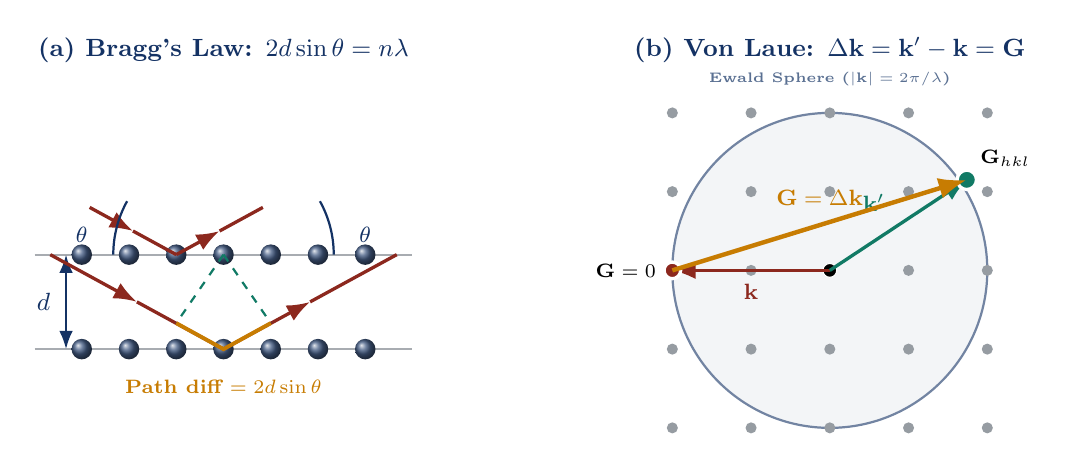
\begin{tikzpicture}[>=Latex]

  % Panel (a): Bragg's Law in Real Space
  \begin{scope}[shift={(0,0)}]
    \node[align=center, font=\bfseries\small, text=primary] at (2.9, 4.8) 
      {(a) Bragg's Law: $2d\sin\theta = n\lambda$};

    % Atomic planes
    \draw[thick, greycol!50] (0.5, 2.2) -- (5.3, 2.2);
    \draw[thick, greycol!50] (0.5, 1.0) -- (5.3, 1.0);

    \foreach \x in {1.1, 1.7, 2.3, 2.9, 3.5, 4.1, 4.7} {
      \shade[ball color=primary!80] (\x, 2.2) circle (0.13);
      \shade[ball color=primary!80] (\x, 1.0) circle (0.13);
    }

    % Spacing d
    \draw[<->, primary, thick] (0.9, 1.0) -- (0.9, 2.2) node[midway, left=2pt, font=\small\bfseries] {$d$};

    % Incident ray 1 reflecting at (2.3, 2.2)
    \draw[->, very thick, secondary] (1.2, 2.8) -- (1.75, 2.5);
    \draw[very thick, secondary] (1.75, 2.5) -- (2.3, 2.2);
    \draw[->, very thick, secondary] (2.3, 2.2) -- (2.85, 2.5);
    \draw[very thick, secondary] (2.85, 2.5) -- (3.4, 2.8);

    % Incident ray 2 reflecting at (2.9, 1.0)
    \draw[->, very thick, secondary] (0.7, 2.2) -- (1.8, 1.6);
    \draw[very thick, secondary] (1.8, 1.6) -- (2.9, 1.0);
    \draw[->, very thick, secondary] (2.9, 1.0) -- (4.0, 1.6);
    \draw[very thick, secondary] (4.0, 1.6) -- (5.1, 2.2);

    % Bragg angle arc
    \draw[thick, primary] (1.5, 2.2) arc (180:151:1.4);
    \node[font=\footnotesize\bfseries, primary] at (1.1, 2.45) {$\theta$};
    \draw[thick, primary] (4.3, 2.2) arc (0:29:1.4);
    \node[font=\footnotesize\bfseries, primary] at (4.7, 2.45) {$\theta$};

    % Path difference perpendiculars
    \coordinate (P) at (2.9, 1.0);
    \draw[dashed, tealcol, thick] (2.9, 2.2) -- (2.3, 1.33) coordinate (D1);
    \draw[dashed, tealcol, thick] (2.9, 2.2) -- (3.5, 1.33) coordinate (D2);
    \draw[line width=1.4pt, orangecol] (D1) -- (P) -- (D2);
    \node[below=2pt, font=\scriptsize\bfseries, orangecol] at (2.9, 0.8) {Path diff $= 2d\sin\theta$};
  \end{scope}

  % Panel (b): Laue Condition & Ewald Sphere
  \begin{scope}[shift={(8.0,0)}]
    \node[align=center, font=\bfseries\small, text=primary] at (2.6, 4.8) 
      {(b) Von Laue: $\Delta\mathbf{k} = \mathbf{k}' - \mathbf{k} = \mathbf{G}$};

    \coordinate (Origin) at (2.6, 2.0);
    \draw[thick, primary!60, fill=primary!5] (Origin) circle (2.0);
    \node[above=2pt, font=\tiny\bfseries, primary!70] at (2.6, 4.15) {Ewald Sphere ($|\mathbf{k}|=2\pi/\lambda$)};

    \foreach \x in {0.6, 1.6, 2.6, 3.6, 4.6} {
      \foreach \y in {0.0, 1.0, 2.0, 3.0, 4.0} {
        \fill[greycol!60] (\x, \y) circle (2pt);
      }
    }

    \filldraw[fill=black, draw=white] (Origin) circle (2.5pt);

    \coordinate (RecipOrigin) at (0.6, 2.0);
    \draw[->, very thick, secondary] (Origin) -- (RecipOrigin) node[midway, below=1pt, font=\footnotesize\bfseries] {$\mathbf{k}$};
    \filldraw[fill=secondary, draw=white, very thick] (RecipOrigin) circle (3pt) node[left=2pt, font=\scriptsize\bfseries] {$\mathbf{G}=0$};

    \coordinate (BraggPoint) at (4.34, 3.15);
    \draw[->, very thick, tealcol] (Origin) -- (BraggPoint) node[midway, above left=1pt, font=\footnotesize\bfseries] {$\mathbf{k}'$};
    \filldraw[fill=tealcol, draw=white, very thick] (BraggPoint) circle (3.5pt) node[above right=1pt, font=\scriptsize\bfseries] {$\mathbf{G}_{hkl}$};

    \draw[->, line width=1.6pt, orangecol] (RecipOrigin) -- (BraggPoint) 
      node[midway, above=3pt, font=\footnotesize\bfseries] {$\mathbf{G} = \Delta\mathbf{k}$};

  \end{scope}

\end{tikzpicture}
\end{document}
